\documentclass{article}
\usepackage{amssymb}
\usepackage{graphicx}
\usepackage{caption}
\usepackage{subcaption}
\usepackage{listings}
\usepackage{float} %figure inside minipage
\graphicspath{ {./images/} }
\usepackage[export]{adjustbox}
\usepackage{apacite}

\begin{document}

\section{Discontinuity in the PDE case}
\subsection{Introduction}
\label{subsection:pde_intro}
In this chapter, we present a similar investigation of solutions to problems with discontinuities in the partial differential equation (PDE) case. To that effect, we will use a 1D PDE epidemiological model similar to those often used in research in that area. 

Again, it is vital that numerical errors associated with the solvers are neglible compared to the modeling errors so that epidemiologist con perform conclusive errors. However, in the PDE case, we often find that rudimentary solvers (often a variation that reduce to using the Euler method) are used. As in the ODE case, it would be very suprising that these solvers are able to reach an accurate solution. To that effect, we spend Section $\ref{subsection:pde_software}$ on introducing BACOLIKR and explaining its importance for the accurate solving of PDE problems. To our knowledge, it is also the only PDE solver capable of event detection which as, shown in the previous chapter, becomes vital for accurate solutions of state-dependent discontinuity problems.

In Section $\ref{subsection:pde_thrashing}$, we reintroduce thrashing for the PDE case, in Section $\ref{subsection:pde_software}$, we provide the BACOLIKR description and in Section $\ref{subsection:pde_problem_def}$, we give a description of the epidemiological model used.

We provide a treatment of the time-dependent discontinuity problem with and without discontinuity handling in Section $\ref{subsection:pde_time_intro}$ and a treatment of the state-dependent discontinuity problem with and without event detection in Section $\ref{subsection:pde_state_intro}$.

\subsubsection{Thrashing in PDE models}
\label{subsection:pde_thrashing}
As was the case with ODE solvers, PDE solvers are also based on mathematical theories that guarantee convergence (a good solution) only when the solution and some of its higher derivatives are continuous. No rigorous mathematical theories guarantee that a PDE solver can solve a discontinuous problems but through experiments, it is known that $\emph{error-control}$ allows solvers to integrate through discontinuities. They do so by repeatedly reducing the step-size until the error of the new step satisfies the user-provided tolerance. Only then is the step accepted.

Thus, when a PDE solver is asked to integrate through a discontinuity, it thrashes. It repeatedly reduces the step-size at that discontinuity until the step-size is small enough to integrate through it. This is observed as a spike in the number of function evaluations at a discontinuity. Figure $\ref{fig:thrashing_pde}$ shows such a phenomenon. A problem with a discontinuity placed at t=30 is solved and we plot the cumulative number of function evaluation at each time interval that the solver, BACOLIKR takes. (We can clearly see the spike at t=30. )
 
\begin{figure}[H]
\centering
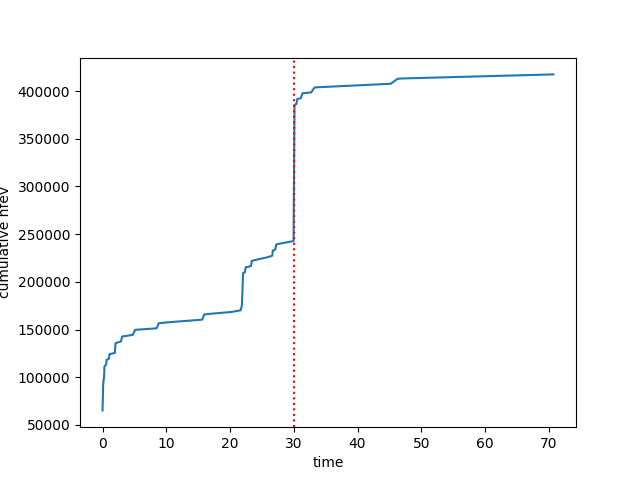
\includegraphics[width=0.7\linewidth]{./figures/pde_thrashing}
\caption{Thrashing in the PDE context}
\label{fig:thrashing_pde}
\end{figure}

In this chapter, we will show that PDE solvers with error-control, like BACOLIKR,  can integrate through one time-dependent discontinuity but that discontinuity handling lead to more efficient solutions as was the case with time-dependent dicontinuous ODE problems (See Section $\ref{subsection:pde_time_intro}$). We will also show that state-dependent discontinuity problems cannot be solved without event detection and that even with event detection, the user will have to be satisfied with an accuracy-efficiency trade-off (See Section $\ref{subsection:pde_state_intro}$).

\subsubsection{BACOLIKR, error-control event detection PDE solver}
\label{subsection:pde_software}
BACOLIKR is a member of the BACOL family of PDE solvers 8888 need reference 8888. Its underlying principle is the same a BACOL in that it solves PDE problems with a spline collocation method using the B-spline bases. 

The collocation process is applied on the spatial dimension to approximate the PDE system with a time-dependent larger ODE system. Using this ODE system and the provided boundary conditions, BACOLIKR produces a time-dependent system of Differential-Algebraic Equations (DAE) which it solves with the DAE solver, DASKR (a modification of DASSL with root-finding) 888 need a reference 888. DASSL provides adaptive time-stepping and adaptive method order selection (chooses an appropriate BDF method). BACOLIKR also provides control over the spatial error throug adaptive refinement of the spatial mesh. 

 
Being an error-control solver, BACOLIKR tries to satisfy a user provided tolerance in the most efficient way possible and by using a root-finding DAE solver like DASKR, BACOLIKR can also perform event-detection and thus can be used for cold starts around discontinuities. We emphasize these two qualities of BACOLIKR as they guarantee accuracy and efficiency that other implementations of PDE solvers, especially rudimentary ones, very rarely grant.

\subsubsection{Problem Definition}
\label{subsection:pde_problem_def}
In this paper, the PDE model we will try to solve is an extension of the SEIR model for epidemiological PDE studies that uses a spatial variable, x, and a time variable, t. Similar PDE models have been used before 8888 reference to PDE Cholera papers 8888 and either use the spread in geographical location or the spread across age groups as the additional spatial variable.

A PDE problem is fully described using a system of partial differential equations of the form:
\begin{equation}
u_t(x, t) = f(x, t, u(x,t), u_x(x,t), u_{xx}(x,t))
\end{equation} 
over a spatial domain ${a \leq x \leq b}$ and an initial time ${t_0}$. 

It requires a set of initial conditions of the form:
\begin{equation}
u(x, t) = u_0(x)
\end{equation}
for x in the spatial domain, ${a \leq x \leq b}$.

It also requires boundary conditions of the form:
\begin{equation}
b_L(t, u(a,t), u_x(a,t)) = 0, b_R(t, u(b,t), u_x(b,t)) = 0 
\end{equation} 
for every time, $t \geq t_0$ .

To that effect, we define an SEIR model based on the one developed by Andrew Fraser 88888 Reference 88888 as follows:

The system of PDEs is:
\begin{equation}
S(x, t)_t = D_S(x)S(x, t)_{xx} + \mu N - \mu S(x, t) - \frac{\beta}{N}S(x, t)I(x, t)
\end{equation}
\begin{equation}
E(x, t)_t = D_E(x)E(x, t)_{xx} + \frac{\beta}{N}S(x, t)I(x, t) - \alpha E(x, t) - \mu E(x, t)
\end{equation}

\begin{equation}
I(x, t)_t = D_I(x)I(x, t)_{xx} + \alpha E(x, t) - \gamma I(x, t) - \mu I(x, t)
\end{equation}

\begin{equation}
R(x, t)_t = D_R(x)R(x, t)_{xx} + \gamma I(x, t) - \mu R(x, t)
\end{equation} 

The spatial domain is $-5 \leq x \leq 5$ and the temporal domain is $0 \leq t \leq 70$ for the time-dependent discontinuity problem but we will use $0 \leq t \leq 200$ for the space-dependent discontinuity problem as we attempt a long-term forecast.

The parameters for the SEIR are as such: $\mu$, the birth rate, is set to $\frac{0.01}{365}$. $\gamma$, the recovery rate is 0.06, $\alpha$, the incubation rate is 0.125 and we will vary the transmission rate, $\beta$, between 0.035 and 0.9 based on whether measures, such as social distancing and others, are implemented or not in the model. The population size, N, is $37*10^{6}$.

The model also uses diffusion functions $D_S(x)$, $D_E(x)$, $D_I(x)$ and $D_R(x)$ to start the infection at a specific point in the spatial domain and spread it over time. These are as follows:
\begin{equation}
D_S(x) = D_E(x) = D_R(x) = (maxD_s - minD_s)e^{-10(\sqrt{x^{2}} - 1)^2)} + minD_s
\end{equation} 
\begin{equation}
D_I(x) = D_E(x)/10
\end{equation}
The diffusivity parameters $maxD_s$ and $minD_s$ are 0.8 and 0.01 respectively. 

\begin{figure}[H]
\centering
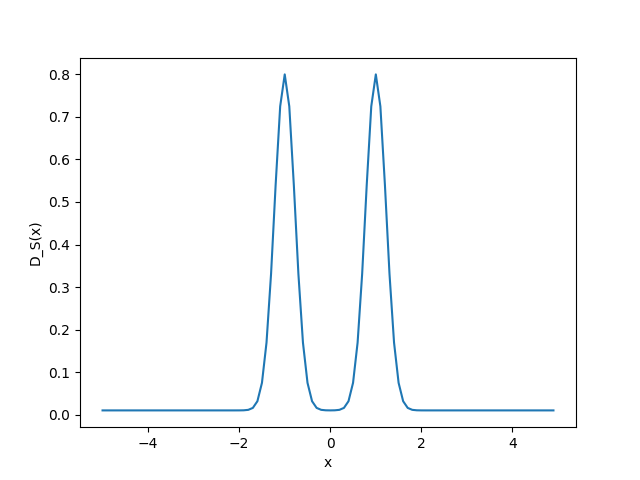
\includegraphics[width=0.7\linewidth]{./figures/pde_D_s}
\caption{Plot of the diffusivity parameter $D_S(x)$}
\label{fig:pde_D_s}
\end{figure}

The set of initial conditions are defined over the spatial domain as such:
\begin{equation}
S(x, 0) = N - I(x, 0)
\end{equation}
\begin{equation}
I(x, 0) = 100e^{-x^2}
\end{equation}
\begin{equation}
E(x, 0) = R(x, 0) = 0
\end{equation}

\begin{figure}[H]
\centering
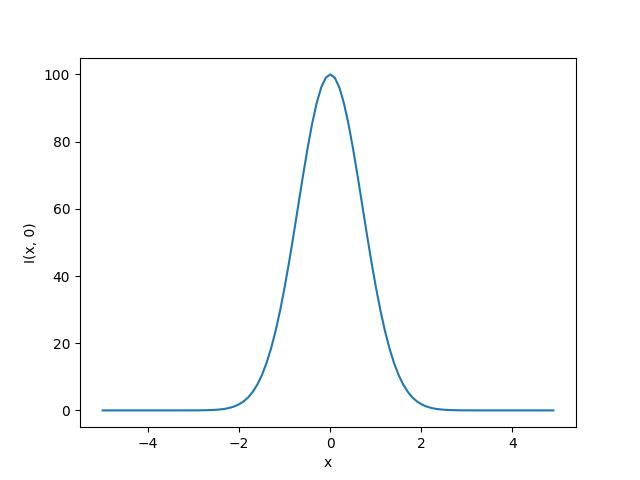
\includegraphics[width=0.7\linewidth]{./figures/pde_I_0}
\caption{Plot of the initial condition I(x, 0)}
\label{fig:pde_I_0}
\end{figure}

We will use the default boundary conditions 888888888888888888 I did not understand what BACOLIKR is doing for the initial conditions here 888888888888888888

The above gives us a complete PDE problem definition. To this problem we will add discontinuities as follows: 
In the time-dependent discontinuity problem, we will integrate the model with $\beta$ at a value of 0.9 from t=0 to t=30, we will then change the value of $\beta$ to 0.035 and integrate until t=70. This change in the parameter introduces a discontinuity. This simulates a scenario where 30 days into a disease, measures are introduced to slow its spread.

In the state-dependent discontinuity problem, we start the integration with the value of $\beta$ at 0.9 until the integral value of the E-component of the solution over the spatial domain at a specific time-step is 30000. When that integral value reaches 30000, we change the value of $\beta$ to 0.035 until the integral value of the E-component over the spatial domain reaches 10000. We then integrate with a value $\beta$ of 0.9. We repeat this process until t=200. This process simulates a series of introducing and relaxing measures, such as social distancing, based on the total number of exposed individuals across the whole region.

\subsection{Time Dependent Discontinuity}
\label{subsection:pde_time_intro}
In this section, we will add a time dependent discontinuity and report on the thrashing experienced by the solvers. We note that this section is in essence an application of what we demonstrated in Section 8888 reference to ODE time dependent 8888 in that time dependent discontinuities are introduced by simply changing a parameter value, as this is essentially changing the model function being integrated and that time-dependent discontinuities have an easy solution by integrating the solution with two calls, one before the discontinuity and one after. This gives the solver two continuous segments to integrate.

In this PDE case, the value of $\beta$ will be 0.9 from t=0 to t=30 and the value of $\beta$ will be changed to 0.035 from t=30 to the end of the integration.

\subsubsection{Naive treatment of the time-dependent discontinuity PDE model}
\label{subsubsection:pde_time_naive}
In the naive treatment for this kind of discontinuity is to place the the change in the parameter in the right hand side function as an if-statement. The pseudo-code for this approach is as follows:

\begin{minipage}{\linewidth}
\begin{lstlisting}[language=Python]
function model_with_if(t, x, u, ux, uxx)
    // ...
    beta = 0.9
    if t >= 30:
        beta = 0.035
    // ...

\end{lstlisting}
\end{minipage}

This change in the parameter $\beta$ at t=30 introduces a discontinuity as the model function is different. As shown in Section 8888 Refer to section on discontinuity 8888, as the assumptions of continuity of the function and its derivatives no longer hold, the Taylor Series proof of its convergence is no longer valid. However as we have shown in Section 8888 Refer to naive ODE time problem 8888, error-control solver can reduce the step-size extensively to cross one discontinuity.


\begin{figure}[H]
\centering
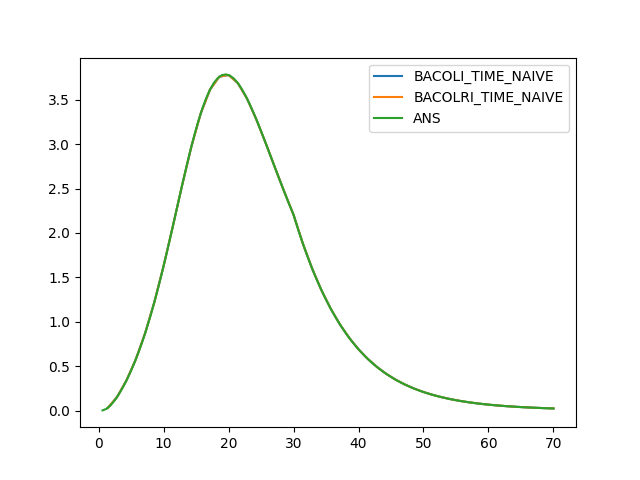
\includegraphics[width=0.7\linewidth]{./figures/pde_time_disc_naive}
\caption{Naive treatment of time discontinuity (at tolerance of $10^{-6}$)}
\label{fig:pde_time_disc_naive}
\end{figure}

From Figure $\ref{fig:pde_time_disc_naive}$, we can see that to eye-level accuracy, the results are accurate. We will now show how a cold start can keep the same level of accuracy while using less function evaluations and thus be more efficient.

\subsubsection{Discontinuity handling to solve the time-dependent PDE model}
\label{subsubsection:pde_time_disc_hand}
Though the error-controlled solvers were able to get accurate solutions, we now solve the same problem using discontinuity handling. Modern solvers like BACOLIKR allows users to set flags to allow it to do a cold start. Thus we integrate the problem with one call from t=0 to t=30 with the model function using 0.9 as the $\beta$ parameter. We then set up a cold start and integrate from t=30 to the end of the time interval with another call to the solver. The pseudo-code is as follows

\begin{minipage}{\linewidth}
\begin{lstlisting}[language=Python]
function model_before(t, x, u, ux, uxx):
    // ...
    beta = 0.9
    // ...
    
function model_after(t, x, u, ux, uxx):
    // ...
    beta = 0.035
    // ...
 
tspan_before = [0, 30]
pde_solver(solution, model_before, tspan_before)

solution.cold_start_flag = True

tspan_after = [30, 70]
pde_solver(solution, model_after, tspan_after)

\end{lstlisting}
\end{minipage}

\begin{figure}[H]
\centering
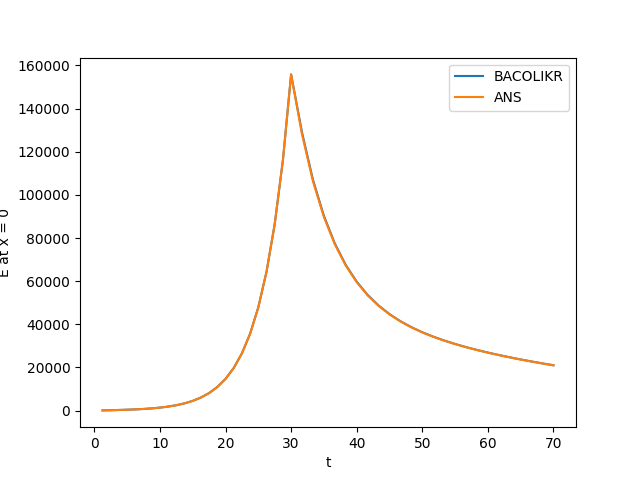
\includegraphics[width=0.7\linewidth]{./figures/pde_time_disc_disc_hand}
\caption{Discontinuity handling for time discontinuity problem (at tolerance of $10^{-6}$)}
\label{fig:pde_time_disc_disc_hand}
\end{figure}

As expected, Figure $\ref{fig:pde_time_disc_disc_hand}$, the solvers were able to all accurately solve the problem. However, Table $\ref{tab:pde_time_nfev}$ shows how the discontinuity handling allows us to use significantly lower numbers of function evaluations.

We note that without the cold start, the solver used 417505 function evaluations. With a cold start the solver uses 359755 function evaluations. We can see that the cold start improved efficiency.

\subsubsection{PDE Time-dependent discontinuity problem tolerance study}
\label{subsubsection:pde_time_tol}
In this section, we do a tolerance study on the time dependent problem. We look at how coarse we can reduce the tolerance to still have accurate solution to see if the discontinuity handling allows us to use coarser tolerance as it did in the IVODE case.

\begin{figure}[H]
\centering
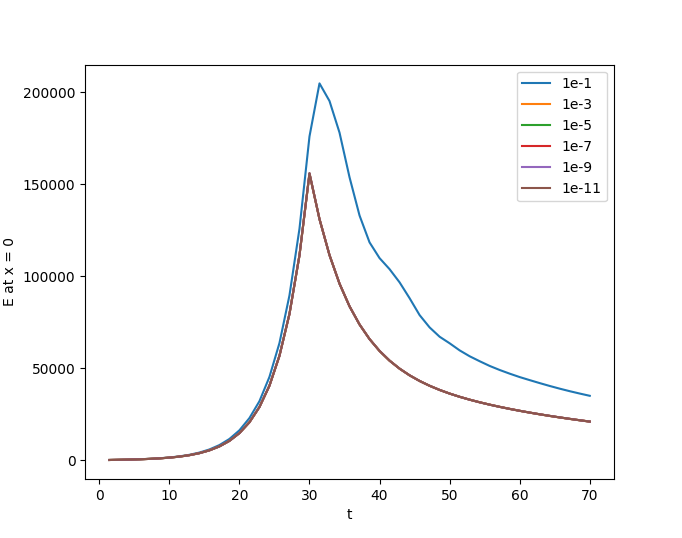
\includegraphics[width=0.7\linewidth]{./figures/pde_time_disc_bacolikr_naive_tol}
\caption{Time dependent discontinuity tolerance study with BACOLIKR without discontinuity handling}
\label{fig:pde_time_disc_bacolikr_naive_tol}
\end{figure}

\begin{figure}[H]
\centering
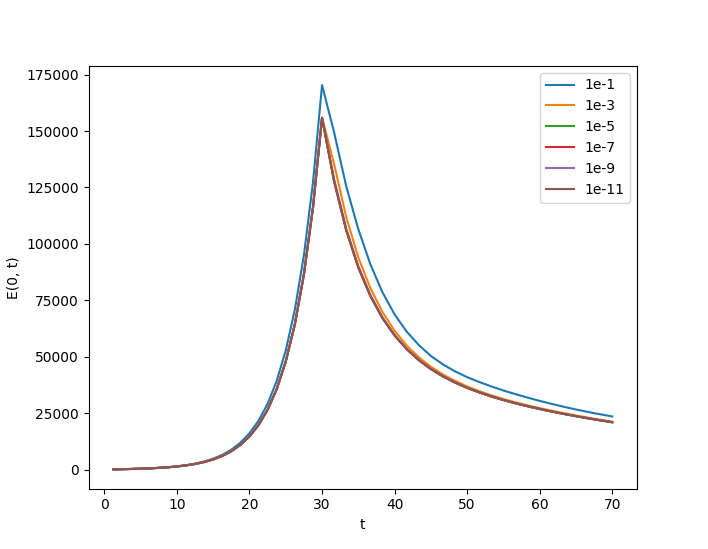
\includegraphics[width=0.7\linewidth]{./figures/pde_time_disc_bacolikr_disc_hand_tol}
\caption{Time dependent discontinuity tolerance study with BACOLIKR using discontinuity handlng}
\label{fig:pde_time_disc_bacolikr_disc_hand_tol}
\end{figure}

\begin{table}[h]
\caption {PDE time discontinuity tolerance study} 
\label{tab:pde_time_nfev}
\begin{center}
\begin{tabular}{ c c c  } 
tolerance & BACOLIKR naive nfev & BACOLIKR disc hand nfev \\ 
1e-1      &   40, 800           &   55, 400   \\
1e-3      &   79, 220           &  76, 750    \\
1e-5      &  206, 980           &  208, 870    \\
1e-7      &  733, 210           &  543, 850     \\
1e-9      & 1, 904, 080         & 1, 653, 830   \\
1e-11     & 7, 140, 875         & 4, 979, 555   \\
\end{tabular}
\end{center}
\end{table} 



\subsection{State Dependent Discontinuity}
\label{subsection:pde_state_intro}
In this section, we discuss a state-dependent discontinuity problem in that we compare the current value of the state or one of its component against a predetermined threshold and if that threshold is crossed, we change the model equation. Unlike, in the IVODE case, we need to account for the spatial domain when finding the state value to compare against a threshold. Some of the ways to do so are listed below:
\begin{itemize}
\item Pick a spatial value, say x = 0, and sample the state value at this spatial point at every time interval. If the state value meets a certain threshold, we apply a different model, else we use the same model

\item Find some statistic measure (min, max, mean, median) across the spatial domain and use that value for the comparison with the threshold.

\item Integrate over the spatial domain and use that integral value for the comparison against the threshold.
\end{itemize}

In this report we will use the third method in that we will integrate over the spatial domain. If the value of the integral crosses a maximum threshold (integral value of 5) while measures are not implemented, the value of the parameter $\beta$ is changed from 0.9 to 0.005 and if measures are implemented and we cross a certain minimum threshold (integral value of 1), the value of the parameter $\beta$ is changed back to 0.9. This is repeated several time for the time period t=0 to t=200.  

We note that the discontinuity is introduced by the change in the parameter $\beta$ and which method to obtain the state value at a certain time does not matter, so the conclusions of this paper equally applies to the other methods of finding the state value at a given time.
 
\subsubsection{Naive treatment of the state-dependent discontinuity model}
\label{subsubsection:pde_state_naive}
For the naive treatment of this problem, a user will use a boolean for whether measures are implemented or not, as a global variable. This global variable is toggled based on the integral value over the spatial domain at a given time.  

To perform the integration the naive user will have to do a manual time stepping. The user will divide the time into equal intervals and once they reach the end of the time interval, they will make an interpolant over the spatial domain at that time and integrate it. 

If measures are not implemented and the integral is greater than 5, the maximum threshold, they will switch the global variable indicating that measures are implemented. When there are no measures implemented, the user will integrate at the end of a step and look for an integral value less than 1, the minimum threshold. When such an integral value is less than 1, the user will switch the global variable indicating that measures are no longer implemented. When measures are implemented, the value of the parameter $\beta$ is 0.005 while it is 0.9 when measures are not implemented. 

The pseudocode for this approach is as shown:

\begin{minipage}{\linewidth}
\begin{lstlisting}[language=Python]
measures_implemented = False

function model(t, x, u, ux, uxx):
    // ...
    if (measures_implemented):
    		beta = 0.035
    	else:
    		beta = 0.9
    // ...

tstart = 0
tstop = 200
num_times = 400
time_step_size = (tstop - tstart) / num_times
		
t_current = tstart
t_next = t_current + time_step_size

while t_current < tstop:
	tspan = [t_current, t_next]
	pde_solver(solution, model, tspan)
	
	integral_value = integrate(interpolate(solution))
	
	if (measures_implemented):
		if (integral_value >= 6):
			measures_implemented = True
	else:
		if (integral_value <= 1):
			measures_implemented = False
	
	t_current = t_next
	t_next = t_next + time_step_size
\end{lstlisting}
\end{minipage}

The pseudo-code shows a clear problem with the naive solution. The user has an additional variable, the number of time steps, to set. The number of time steps needs to be big enough that we know when the threshold are met but need to be small enough that the integration can occur without issue. 

The solution on solving this problem with a naive solution is as shown in Figures 8888 8888 and 8888 8888 where the number of time steps is 200 and 400 respectively. 

\begin{figure}[H]
\centering
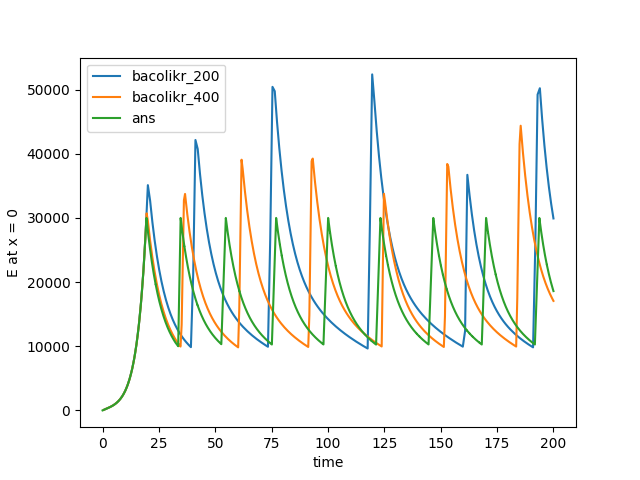
\includegraphics[width=0.7\linewidth]{./figures/pde_state_disc_naive_200vs400}
\caption{State dependent discontinuity naive treatment with a tolerance of $10^{-6}$ and 200 vs 400 time steps}
\label{fig:pde_state_disc_naive_200vs400}
\end{figure}

\subsubsection{Why the naive method cannot give an accurate solution}
\label{subsubsection:pde_state_naive_always_inaccurate}
The naive method cannot solve the problem accurately because of the problem of choosing a correct number of time steps to perform the spatial integration. We note that most of the time, the method will find the correct integral value much after it crosses the threshold and not exactly when it does so. This means that we take up to one additional time step with the previous $\beta$ value and not the correct one.

One idea to solve this problem would be to use an exceedingly large number of time steps (1000 in our case) such that we take the smallest step possible with the old value. This, however, reduces the efficiency, making us do more time steps than necessary. (See efficiency comparisons in Table 8888 Refer to table in next section 8888). The best solution is to use event detection.

\begin{figure}[H]
\centering
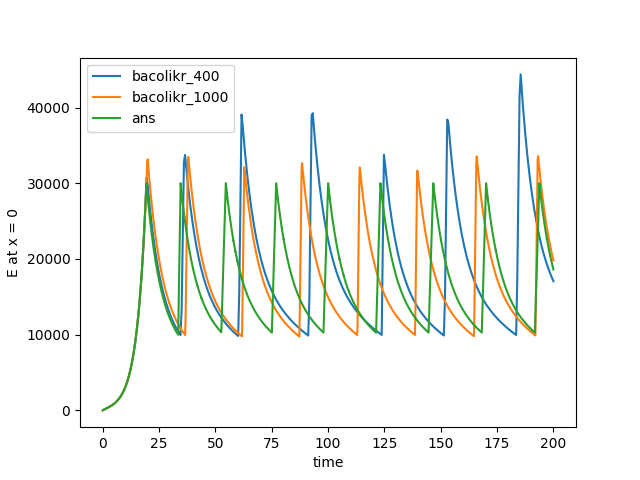
\includegraphics[width=0.7\linewidth]{./figures/pde_state_disc_naive_400vs1000}
\caption{State dependent discontinuity naive treatment with a tolerance of $10^{-6}$ and 400vs1000 time steps}
\label{fig:pde_state_disc_naive_400vs1000}
\end{figure}
 
From the above, we can see that a high enough number of time steps allow us to get better and better solution...

\subsubsection{Event Detection solution to the naive state-dependent discontinuity model}
\label{subsubsection:pde_state_event_detection}
As was the case in the IVODE case, event detection is also present in some PDE solvers. Event detection works in the same way: the user provides a root function to the PDE solver, after each time step the solver calls the root function with the solution at the current time step and stores its value. If the value returned by the root function changes sign, the PDE solvers employs a root-finding routine to find where the root function is zero exactly. The solver then returns, setting a flags indicating that it has found a root with the values at the root.
 
BACOLIKR is an improvement to the BACOLI solver which has root finding capabilities. Instead of using DASSL as its DAE solver, it uses DASKR which can detect roots as its solves a DAE system. We use BACOLIKR to demonstrate that using a PDE SOLVER with root-finding capabilities allows us to not define a time grid and thus allows us to integrate with the best accuracy-efficiency trade-off.  

We define two pairs of root and model functions. One pair is to be used when integrating when there are no measures in place. The model function will have the variable $\beta$ at a value of 0.9 and the root function will do the integration of the spatial domain at the current time step and will return if it is closed to the maximum threshold. 5. The second pair will have the model function with $\beta$ at a value of 0.035 and the root function looking for a root at 1. The pseudo-code for this approach is as follows:

\begin{minipage}{\linewidth}
\begin{lstlisting}[language=Python]
function model_no_measures(t, x, u, ux, uxx):
	// ...
	beta = 0.9
	// ...
	
function root_max_value(t, solution):
	// ...
	integral_value = integrate(interpolate(solution))
	return integral_value - 5
	
function model_with_measures(t, x, u, ux, uxx):
	// ...
	beta = 0.035
	// ...
	
function root_min_value(t, solution):
	// ...
	integral_value = integrate(interpolate(solution))
	return integral_value - 1


tstart = 0
tstop = 200
		
t_current = tstart
measures_implemented = false

while t_current < tstop:
	tspan = [t_current, t_stop]
	if (measures_implemented):
		pde_solver(solution, model_with_measures, tspan, root_min_value)
	else:
		pde_solver(solution, model_no_measures, tspan, root_max_value)
		
	if (solution.root_flag == True):
		# root detected, if a max root, add measures else remove measures
		solution.cold_start_flag = True
		if (measures_implemented):
			measures_implemented = False
		else:
			measures_implemented = True
		
	t_current = solution.t

\end{lstlisting}
\end{minipage}


\begin{figure}[H]
\centering
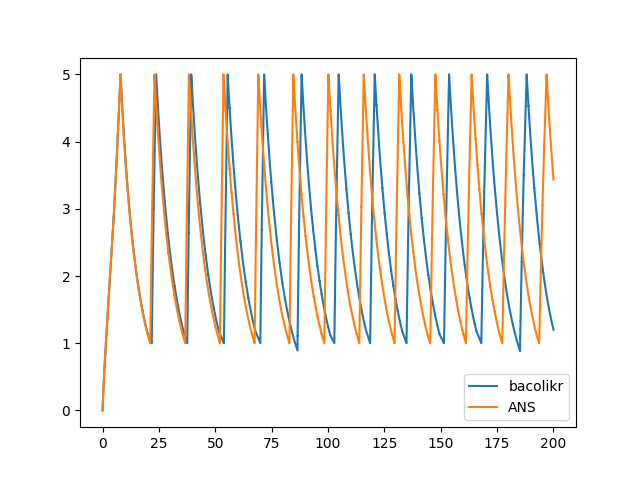
\includegraphics[width=0.7\linewidth]{./figures/pde_state_disc_event_tol_6}
\caption{State dependent discontinuity using event detection with a tolerance of $10^{-6}$}
\label{fig:pde_state_disc_event_tol_6}
\end{figure}

As we can see, we get a solution that oscillates correctly. However the two solutions are not correctly aligned, especially at lower time period. We will see that the tolerance need to be high enough

\begin{figure}[H]
\centering
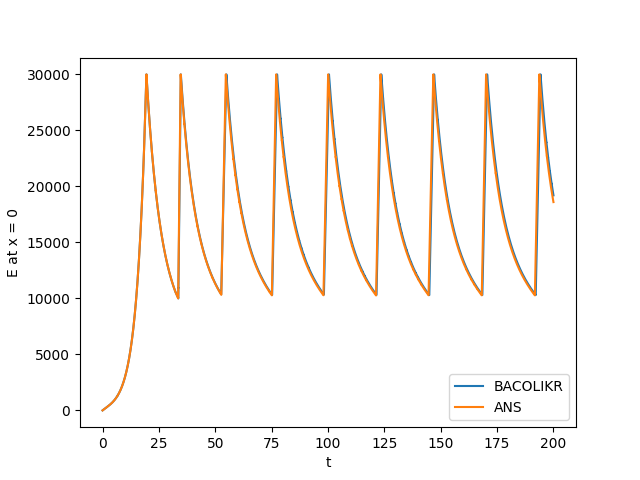
\includegraphics[width=0.7\linewidth]{./figures/pde_state_disc_event_tol_9}
\caption{State dependent discontinuity using event detection with a tolerance of $10^{-9}$}
\label{fig:pde_state_disc_event_tol_9}
\end{figure}

From Figures $\ref{fig:pde_state_disc_event_tol_6}$ and $\ref{fig:pde_state_disc_event_tol_9}$, we can see that with event detection, it is only a matter of tolerance to see whether the answer is accurate. We note that this might be because of how the root finding works. A stricter tolerance at the root makes DASKR stop closer to the root and thus begin with a different $\beta$ value.

\begin{table}[h]
\caption {PDE state discontinuity model} 
\label{tab:pde_state_nfev}
\begin{center}
\begin{tabular}{ c c } 
method                    & nfev \\ 
BACOLIKR naive 200 steps  & 1, 018, 455    \\
BACOLIKR naive 400 steps  & 1, 184, 880    \\
BACOLIKR naive 1000 steps & 1, 280, 080    \\
BACOLIKR $10^{-6}$ tol.   & 1, 937, 730    \\
BACOLIKR $10^{-9}$ tol.   & 7, 915, 085    \\
\end{tabular}
\end{center}
\end{table}

Table $\ref{tab:pde_state_nfev}$ starts showing the pattern for the PDE state discontinuity. The problem is a trade-off between efficiency and accuracy even with root-finding. Improving the accuracy comes at the price of efficiency. We note that without event detection, the solutions even with 1000 time steps are still inaccurate. The solutions never oscillate correctly between 10, 000 and 30, 000. However, even with event detection, the tolerance needs to be high enough to get accurate solutions.

\subsubsection{State problem tolerance study}
\label{subsubsection:pde_state_tol_study}
We also perform a tolerance study at 400 and at 1000 to show how the solutions compare for all the solvers. We try to look for why even BACOLIKR does not solve the problem and look to see if there is anything we can do

\paragraph{BACOLIKR without event}
\begin{figure}[H]
\centering
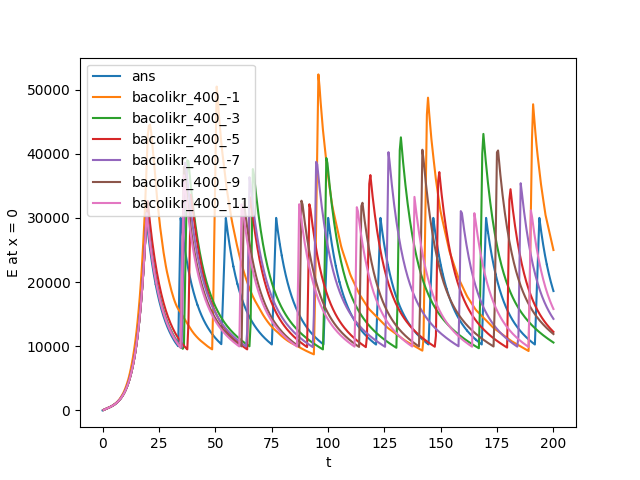
\includegraphics[width=0.7\linewidth]{./figures/pde_state_disc_tol_bacolikr_naive_400}
\caption{State dependent discontinuity naive treatment tolerance study with BACOLIKR with 400 time steps}
\label{fig:pde_state_disc_tol_bacolikr_naive_400}
\end{figure}

\begin{figure}[H]
\centering
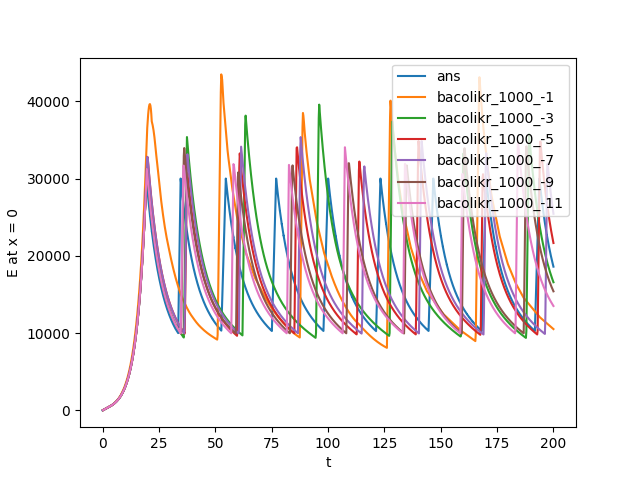
\includegraphics[width=0.7\linewidth]{./figures/pde_state_disc_tol_bacolikr_naive_1000}
\caption{State dependent discontinuity naive treatment tolerance study with BACOLIKR with 1000 time steps}
\label{fig:pde_state_disc_tol_bacolikr_naive_1000}
\end{figure}

Figures $\ref{fig:pde_state_disc_tol_bacolikr_naive_400}$ and $\ref{fig:pde_state_disc_tol_bacolikr_naive_1000}$ show that the solutions are not aligned and the roots are not detected exactly at 30000 in the case without event detection. We note that the problem is mostly in the exponentially increasing direction due to the instability. Having a higher time step slightly improves the situation but we will see that with event detection improves the accuracy to a greater degree.

\paragraph{BACOLIKR with event detection}
\begin{figure}[H]
\centering
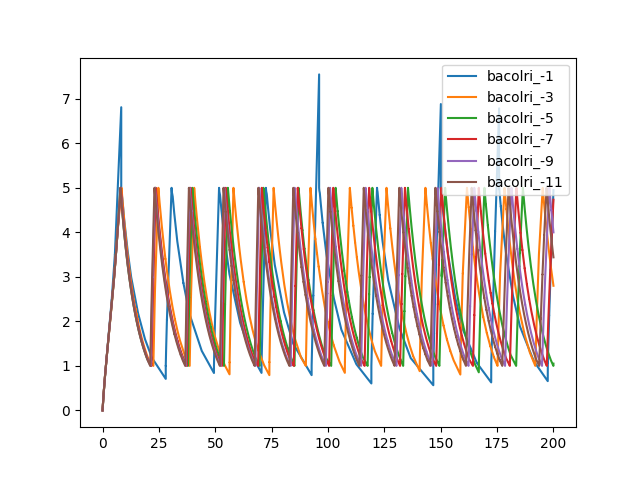
\includegraphics[width=0.7\linewidth]{./figures/pde_state_disc_tol_event}
\caption{State dependent discontinuity using event detection tolerance study}
\label{fig:pde_state_disc_tol_event}
\end{figure}

With event detection, the solution oscillate correctly for all tolerances except at $10^{-1}$. The other solutions are only slightly misaligned but this can be explainined with the tolerance at the roots. Depending on the tolerance, the root is detected at a different time step and thus different tolerances will lead to initiating the next steps of the integral with a different $\beta$ value and thus the solutions are not aligned. 

\paragraph{Efficiency of the solvers}
\begin{table}[h]
\caption {State dependent discontinuity model tolerance study} 
\label{tab:pde_state_tol_study}
\begin{center}
\begin{tabular}{ c c c c } 
tolerance  & BACOLIKR  with event & BACOLIKR naive 400 & BACOLIKR naive 1000 \\ 
1e-1       & 137, 300             & 104, 700           & 101, 250  \\
1e-3       & 376, 855             & 239, 445           & 290, 600  \\
1e-5       & 1, 052, 920          & 736, 360           & 848, 080\\
1e-7       & 3, 217, 450          & 2, 032, 330        & 2, 217, 610 \\
1e-9       & 7, 915, 085          & 5, 236, 500        & 6, 040, 485\\
1e-11      & 21, 256, 400         & 16, 845, 765       & 16, 402, 140  \\
\end{tabular}
\end{center}
\end{table}

Table $\ref{tab:pde_state_tol_study}$ shows that we are forced to sacrifice efficiency for accuracy in this problem. We note that all naive solutions highly depend on the time stepping and thus should not be trusted for accurate solutions. For the solutions using event detection, the accuracy problem is at the roots where the models are to be changed. Depending on the tolerance, the root is detected at a different location as the root-finding algorithm returns the location of the root based on the tolerance. Thus different tolerances will lead to changing the models at slightly different positions. During the exponential increase phase, we can miss the location of the root by far enough that the solutions are not aligned.

\subsection{Discussions}
\label{subsection:pde_discussions}

\end{document}
